\documentclass[12pt]{article}
\usepackage[spanish]{babel}
\usepackage{float}
\usepackage{graphicx}
\usepackage{geometry}
\geometry{
 a4paper,
 left=20mm,
 top=15mm,
 right=20mm,
 bottom=15mm
 }
\usepackage{hyperref}
\usepackage{lipsum}
\usepackage{tgschola}
\usepackage[T1]{fontenc}
\usepackage{multirow}
\usepackage{amsmath}
\usepackage{fancyhdr}
\usepackage{xcolor}
\usepackage{fontawesome}
\definecolor{modcolour}{gray}{0.6}
\usepackage[none]{hyphenat}
\hypersetup{
   colorlinks=true,
   linkcolor=black,
   urlcolor=blue,
}
\urlstyle{same}
\renewcommand{\contentsname}{Índice}
\setlength{\parskip}{0.5em}

\pagestyle{fancy}

\title{Curriculum Vitae}
\author{Damián Ariel Ponce}

\renewcommand{\headrulewidth}{0pt}
\cfoot{}
% Se actualiza solo yay :D
\rfoot{}

\begin{document}

   \noindent
   \begin{tabular}[t]{l@{}} 
     \hspace{-2mm}\multirow{4}{*}{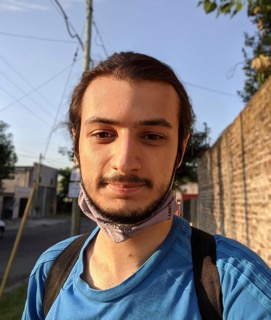
\includegraphics[height=4.5cm]{headshot.jpeg}}
   \end{tabular}\hspace{.3cm}
   \begin{tabular}[t]{@{}c @{  }l} 
   \faMapMarker & ~Morón, Buenos Aires\\[.2cm]
   \faPhone & ~+54 9 11 3429 0789\\[.2cm]
   \faEnvelope & ~\href{mailto:dami.ponce8@gmail.com}{dami.ponce8@gmail.com}\\[.2cm]
   \faLinkedin & ~\href{https://www.linkedin.com/in/damianponce/}{linkedin.com/in/damianponce}\\[.2cm]
   \faGlobe & ~\href{https://damiponce.github.io/}{damiponce.co}\\[.2cm]
   \faBirthdayCake & ~20 años\\

   \\
   \end{tabular}
   \hfill% move it to the right
   \hspace{-2.5cm}
   \begin{tabular}[t]{r@{}} 
   \\[.2cm]
   \\[.2cm]
   \\[.2cm]
   \\
   \\
   \\
   \textbf{\Huge Damián Ariel Ponce}\\
      
   \end{tabular}
   
   % MAYBE REMOVE \noindent
   {\noindent\hrulefill\hspace{-30mm}}

   %%%%%%%%%%%%%%%%%%%%%%%%%%%%
   \vspace{0.5\baselineskip}\noindent
   \renewcommand{\arraystretch}{1}%
   \begin{tabular}[t]{@{}p{1.15in} @{}p{5.35in}}
   
   %%%%%%%%%%%%%%%%%%%%%%%%%%%%
   {\scshape Educación}
   &
   \textbf{Universidad Tecnológica Nacional (FRH)}  \hfill Haedo, Bs.As.\vspace{0.015in} \\ &
   Ingeniería Aeronáutica -- 2do año \hfill 2021 -- Actualidad\vspace{0.015in}
   \vspace{0.7\baselineskip}
   \\
   & \textbf{I.N.A.C. C.I.A.T.A.}  \hfill Morón, Bs.As.\vspace{0.015in} \\ &
   Secundario completo -- Técnico Aviónico \hfill 2014 -- 2020\vspace{0.015in}
   \\
   &
   \vspace{.3\baselineskip}
   {\noindent\hspace{-50mm}\hrulefill}
   \vspace{.7\baselineskip}
   \\
      
   

 %%%%%%%%%%%%%%%%%%%%%%%%%%%%
   {\scshape Proyectos}
   &
   \textbf{Estadísticas de WhatsApp} \href{https://damiponce.github.io/chat-analyser/}{\small(link)}
   \\
   %{\scshape (página web)}
   &
   Herramienta de análisis de datos para chats de Whatsapp.
   \vspace{0.7\baselineskip}
   \\
   & \textbf{Portfolio web} \href{https://damiponce.github.io/}{\small(link)}
   \\
   & Una página donde muestro mis proyectos de manera detallada.
   \vspace{0.7\baselineskip}
   \\
   & \textbf{Animaciones 3D de ruido Perlin} \href{https://damiponce.github.io/3d-noise/}{\small(link)}
   \\
   & Demostración visual de renderizado 3D a tiempo real en el buscador.
   \vspace{0.7\baselineskip}
   \\
   & \textbf{Visualización del clima} \href{https://damiponce.github.io/weather-web/}{\small(link)}
   \\
   & Muestra interactiva de datos meteorológicos de una API open-source.
   \\
   &
   \vspace{.3\baselineskip}
   {\noindent\hspace{-50mm}\hrulefill}
   \vspace{.7\baselineskip}
   \\

   %%%%%%%%%%%%%%%%%%%%%%%%%%%%
   {\scshape Habilidades}
   &
   \textbf{Lenguajes de programación: }  HTML, CSS, SASS, JavaScript, TypeScript, Python.%, LaTeX, Python.
   \vspace{0.7\baselineskip}
   \\
   &
   \textbf{Frameworks de programación: }  Node.js, React, React Native.%, LaTeX, Python.
   \vspace{0.7\baselineskip}
   \\
   &
   \textbf{Herramientas: }  Git, GitHub, Postman, Photoshop, Illustrator, Figma.%, LaTeX, Python.
   \\ 
   %\vspace{0.5\baselineskip}
   %&
   %\textbf{Aplicaciones: }  Desarrollo web (front-end), diseño gráfico, edición de %imagenes y documentación.%, dibujo CAD 2D/3D y formateo de texto.
   %\\
   &
   \vspace{.3\baselineskip}
   {\noindent\hspace{-50mm}\hrulefill}
   \vspace{.7\baselineskip}
   \\
%  &
%  \textbf{Software: }  Microsoft Office (Word, Excel, Powerpoint), Photoshop, %  &  Illustrator, Lightroom, AutoCAD, Inventor, Visual Studio Code.
%  \\
%  \vspace{1\baselineskip}
%  \\

   %%%%%%%%%%%%%%%%%%%%%%%%%%%%
   {\scshape Idiomas}
   &
   \textbf{Español: }  Nativo. \hspace{3cm} \textbf{Ingles: }  Fluído.
   %\vspace{0.7\baselineskip}
   \\
   %&
   %\textbf{Ingles: }  Fluído.
   %\\
   &
   \vspace{.3\baselineskip}
   {\noindent\hspace{-50mm}\hrulefill}
   \vspace{.7\baselineskip}
   \\
   
%%%%%%%%%%%%%%%%%%%%%%%%%%%%
   {\scshape Experiencias}
   &
   \textbf{NASA Space Apps Challenge 2019}  \hfill Morón, Bs.As.\vspace{0.015in} \\ 
   {\scshape Académicas} % ???????????
   & Nominación global del proyecto\hfill Octubre 2019\vspace{0.015in}
   \vspace{0.7\baselineskip}
   \\
   & \textbf{Olimpiada Nacional ONIET N$^{\circ}$23}  \hfill Córdoba, Cba.\vspace{0.015in} \\ &
   4to puesto en la competencia grupal de Electrónica \hfill Octubre 2018\vspace{0.015in}
   \\ 
   &
   \vspace{.3\baselineskip}
   {\noindent\hspace{-50mm}\hrulefill}
   \vspace{.7\baselineskip}
   \\
   %%%%%%%%%%%%%%%%%%%%%%%%%%%%
   {\scshape Cursos}
   &
   \textbf{Radioaficionados}  \hfill Morón, Bs.As.\vspace{0.015in} \\ 
   & I.N.A.C. C.I.A.T.A. \hfill 2018\vspace{0.015in}
   \vspace{0.7\baselineskip}
   \\
   & \textbf{Introducción a Sensores}  \hfill Morón, Bs.As.\vspace{0.015in} \\ &
   I.N.A.C. C.I.A.T.A. -- ifm electronics \hfill 2017\vspace{0.015in}
   \\

   \end{tabular}

\end{document}